%Chapter 4

\renewcommand{\thechapter}{4}

\chapter{Federated Consistency}
\label{ch:federated_consistency}
% Overview, details, consistency, performance, lessons learned.

The next generation of globally distributed systems will not only reside in carefully managed cloud data centers connected by multiple communication trunks.
To handle increasing mobile demand, application services have migrated closer to the edge of the computing environment~\cite{edge_computing}.
Non-human users and machine-to-machine communication will also require geography-specific data systems to handle traffic coordination and electrical grid data~\cite{cisco_internet_trends,sensor_networks,smart_grid,sotis,iot}.
To support these trends, a fog of partial-replicas that serve clients in specific extra-datacenter locations is required to bridge the gap between the centralizing tendency of the cloud and the decentralizing tendency of edge computing~\cite{fog,fog_mobile,fog_iot}.
For that reason, we propose that in addition to first tier strong-consistency backbone, a planetary-scale distributed system also requires a second-tier dissemination network that provides a high-availability mesh between quorum decision making~\cite{oceanstore}.

Outside of a data center context, strong coordination using consensus is simply not feasible~\cite{sensor_coordination}.
In a stable network environment, systems are able to adapt consistency at runtime~\cite{chihoub_harmony:_2012,chihoub_consistency_2013,kraska_consistency_2009,pitoura_data_1999,deno-toc}.
Systems outside of this context are expected to have heterogenous hardware which leads to variability both in terms of capacity and failure rates.
The farther the network diameter, the more partition prone a network becomes, and the higher latencies are experienced between nodes.
Mobility also means dynamic membership with many peers, therefore even adaptable configuration provided by hierarchical consensus is not sufficient.
Taken together, these challenges require a minimization of coordination, instead a focus on cacheing and a high-throughput of writes to the rest of the system.
In other words, a relaxation of consistency guarantees in the fog layer.

In this chapter, we present a novel approach to flexible consistency that federates replicas that participate in a system with different consistency guarantees.
By allowing individual replicas to maintain strong consistency for their clients if they are part of a strongly connected part of the network (e.g. in a datacenter or in the cloud) or to relax consistency guarantees if they are in a more variable network, we ensure that the entire system behaves as a single, integrated entity.
Individual replicas in the system are allowed to adapt to a changing network environment while providing as strong a local guarantee or minimum quality of service as required.
The global state of a federated system is defined by the replica topology and their interactions.
If a subset of replicas implement strong consistency models such has hierarchical consensus, then the global probability of conflict is reduced.
Conversely, a subset of replicas implementing weaker consistency can increase global throughput.
We find that it is more often the tension between local vs. global views of consistency that cause the greatest concerns about application performance.
Because each node can select and change local consistency policies, client applications local to the replica server have greater control of tuning consistency, maximizing timeliness or correctness as needed.

A federated consistency protocol can find a middle ground in the trade-off between performance and consistency.
In this chapter we consider two extremes: an eventually consistent system implemented with gossip-based anti-entropy~\cite{anti_entropy,dynamo} and a sequential consistency model as implemented by the Raft consensus prtocol~\cite{raft} (we use Raft as a stand-in for hierarchical consensus to simplify the discussion in this chapter).
By exploring these two extremes in the consistency spectrum we show that the overall number of inconsistencies in the system is reduced over a homogenous eventual system, and that the access latency is decreased from the homogenous sequential system.

\section{Hybrid Consistency}
\label{ch04_hybrid_consistency}

Federating replicas that participate in multiple protocols leading to different consistency levels creates a \emph{hybrid consistency} model~\cite{hybrid_consistency}.
Hybrid consistency models attempt to use strong consistency with application semantics demand it and weak consistency when not required.
We propose a hybridization not due to required semantics, but rather based on network environment.
Our consistency model is therefore topology-dependent and more than simply hybridizing consistency, can be said to have flexible or dynamic consistency.
We have found that large systems with variable latency in different geographic regions can perform well by allowing most nodes to operate optimistically, but also maintaining a strong central quorum to reduce the amount of global conflict.

In \S~\ref{ch02_consistency} we defined a data-centric consistency model that viewed consistency in terms of per-replica logs that describe the sequence of operations that modify a replica's state.
Consistency models express the correctness of a system based on two metrics: the strictness of log ordering and how stale a log is allowed to be~\cite{bermbach_consistency_2013}.
\emph{Ordering} refers to how closely individual logs adhere to an abstract global ordering.
Strong consistency requires all logs to be identically ordered, and consensus algorithms coordinate a majority of replicas to correctly appended entries to the log in the same order.
Weak consistency allows divergence of the order operations applied to the log.

On the other hand, \emph{Staleness} refers to how far local logs are behind the latest version of the global log, which can be expressed by the average latency of replicating updates, or how far behind the average replica is from the log.
Most data-centric models do not consider staleness, instead referring to guarantees on ordering strictness.
However, the symptoms of inconsistency are primarily due to staleness~\cite{probabilistically_bounded_staleness,quantifying_pbs}.

Consider a system where each update creates a new version of the object that maintains the parent version the update was created from.
In a distributed system with multiple nodes, two forms of inconsistencies can occur.
First, a \emph{stale read} occurs if the version read is not the latest global version, e.g. it is incorrect that reading from two parts of the system may return different answers.
Second, stale reads lead to \emph{forks} on updates: when two replicas concurrently write a new version to the same parent object.
Forks introduce inconsistency because they allow multiple potential orderings of operation logs and from the client's perspective, because they introduce conflicts.

Object \emph{coherence} requires an objects' version history to be a linear sequence~\cite{rethinking_eventual}, which demonstrates that the
system was in a consistent state during all accesses.
Version history forks violate coherence and occur, for example, when replicas $i$ and $j$ read object version $a_1$ then concurrently attempt to write new versions: $W_i(a_1 \rightarrow a_2)$ and $W_j(a_q \rightarrow a_3)$ as shown in Figure~\ref{fig:ch04_forked_writes}.
A delay in synchronization between $R_i$ and $R_j$ could lead one replica to continue farther down the fork paths, e.g. $W_i(a_2 \rightarrow a_4)$.
Forks can be caused by concurrent reads, but the fork between $a_2$ and $a_3$ actually occurs because $R_j$'s read is stale.
Forks are a useful model for exposing how ordering and staleness are considered in different consistency approaches.

\begin{figure}
    \begin{center}
        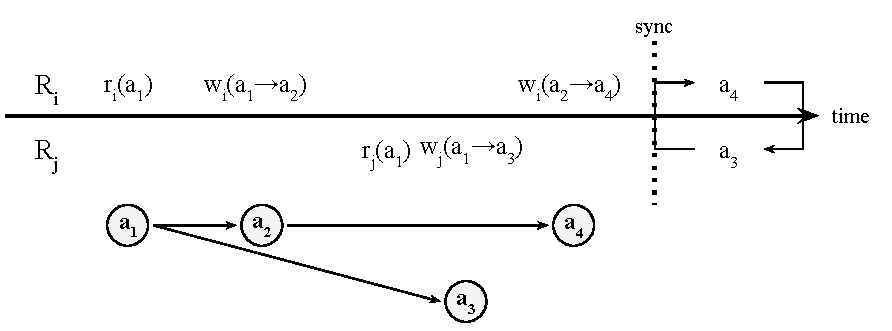
\includegraphics[width=5in]{figures/ch04_forked_writes.pdf}
    \end{center}
    \renewcommand{\baselinestretch}{1}
    \small\normalsize

    \begin{quote}
        \caption[Forked Writes]{Accesses before synchronization cause stale reads and forked writes. In this case if $R_i$ and $R_j$ both attempt to write object a at version 1, $a_1$, the result will be two new versions, $a_2$ and $a_3$ both of which have the parent version $a_1$, which could mean a potential conflict.}
        \label{fig:ch04_forked_writes}
    \end{quote}
\end{figure}
\renewcommand{\baselinestretch}{2}
\small\normalsize

% Additional version metadata, including the parent version of the update (in a
% read-then-write system or simply the latest version of the key stored
% locally), implements a virtual object history that allows us to reason about
% consistency.
% Keys can be managed independently, e.g. each key has its own update id
% sequence resulting in per-object consistency, or all objects can be managed
% together with a single sequence; in the latter case, it is possible to
% construct an ordering history of operations to all objects and in the former,
% a sequence of operations for each object.
% Object histories allow us to reason about the global consistency of the
% system as described in \S~\ref{ch04_hybrid_consistency}.

In an \emph{eventually consistent} system, a replica's log does not depend on any other replica's log except that the last entry appended must eventually be identical for each object in the namespace.
In practice, this means that eventually consistent logs keep track of monotonically increasing versions and that not all versions are required to be present in the log, so long as the same final state is achieved.
This suggests that eventual consistency requires a synchronization mechanism to propagate writes asynchronously and a policy to handle convergence~\cite{bayou}.
Forks occur in the eventually consistent model because it optimistically accepts writes without very much coordination, allowing to concurrent versions to be appended to two different logs.
Generally speaking, conflict resolution is left to the application layer, but in practice each conflict must be resolved as it reaches each replica.

Eventually consistency convergence is typically implemented by a \emph{last writer wins policy}.
When replicas synchronize, they compare the latest version of each object based on all updates prior to their synchronization, then accept whichever version is latest.
As a result, eventually consistent logs may temporarily diverge, so long as the final version of objects eventually converge.
It is therefore acceptable to alternate between writes to competing forks (a fairly weak semantic) or to drop a branch with more updates in favor of a more recent, shorter branch.
In \S~\ref{ch04_anti_entropy} we will describe in more detail the likelihood of forks in bilateral anti-entropy.

In a \emph{sequentially consistent} system, the ordering of updates to individual objects must be identical and no versions must be missing.
However, it is possible that the logs of lagging replicas may only be prefixes of the latest log in the system~\cite{raynal_sequential_2002}.
Sequential consistency therefore does not make guarantees about staleness (or the ordering of reads) but does require all writes become visible in the same order~\cite{bermbach_consistency_2013}.
Sequential consistency can be implemented with consensus algorithms such as Paxos~\cite{paxos} or Raft~\cite{raft}, which coordinate logs by defining a transitive global ordering for all conflicts.
Alternatively, sequential consistency can be implemented with warranties -- time-based assertions about groups of objects that must be met on all replicas before the assertions expire~\cite{liu_warranties_2014}.
In both implementations, forks can be immediately observed because sequential consistency requires coordination when any update occurs.

Stale reads in a sequentially consistent system are possible because of lagging replicas.
However, only a single branch of a forked write can be committed to any copy of the log.
Preventing forks would require either a locking mechanism or an optimistic approach that allowed operations to occur but rejects all but one branch.
Therefore in a sequentially consistent system implemented by consensus, forks are rejected and appear to the user as dropped writes, at which point the client must retry or immediately resolve conflicts.
In \S~\ref{ch04_consensus} we investigate cache read policies for consensus that modulate the probability of a dropped write.

At both ends of the consistency spectrum we have presented, eventual and sequential consistency, it is clear that flexibility is primarily in the \emph{amount} of forks that may occur.
In a hybrid model, we therefore express consistency as a likelihood that a fork occurs.
If a client accesses a strong consistency replica, the likelihood is low and the client is immediately notified of a conflict.
If the access is to an eventually consistent replica, the likelihood is higher, and conflicts must be handled after the access.
Our key insight is that eventually consistent replicas participating in a federated system do not affect the likelihood or behavior of consistency at sequentially consistent replicas.
Although we have discussed strong and weak consistency models, this observation also applies to other consistency models such as causal consistency~\cite{causal,causal_2,cops,bailis_bolt-causal_2013}, for simplicity however, we continue our discussion with only strong and weak models.

\section{Replication}
\label{ch04_replication}

A federated consistency model allows individual replicas to engage in replication according to locally-specified consistency policies.
Each replica maintains its own local state, modified in response to local accesses and receipt of messages from remote replicas.
Each replica sends messages to other replicas to propagate new writes.
Every federated replica must have the ability to handle all types of RPC messages required by different protocols and each protocol must be expressed by separate RPC endpoints.
So long as this is true, then federation primarily has to be defined at the \emph{consistency boundaries}, that is when replicas of one consistency type send messages to that of another.

We consider a system where clients can \texttt{Put} values (write) and \texttt{Get} (read) independent objects specified by a key.
\texttt{Get} requests are fulfilled by reading from the local cache of a replica depending on its read policy.
On \texttt{Put}, a new instance of the object is created and assigned a monotonically increasing, conflict-free \textit{version
number}~\cite{version_conflict_detection,version_vectors}.
For simplicity, we assume a fixed number of replicas, therefore each version is made up of two components: the \textit{update} and \textit{precedence ids}.
Precedence ids are assigned to replicas during configuration, and update ids are incremented to the largest observed value during synchronization.
As a result, any two versions generated by a \texttt{Put} anywhere in the system are comparable such that the \textit{latest} version of the key-value pair is the version with the largest update id, and in the case of ties, the largest precedence id.

For simplicity, we assume that all object instances must become fully replicated to the entire system.
In practice we observe that metadata about the objects usually becomes fully replicated, which points to the locations the object data is stored for retrieval.
Consistency models define how replication occurs.
An eventually consistent model propagates updates asynchronously using gossip-based anti-entropy to synchronize pairs of replicas without congesting the network with broadcasts.
Consensus, on the other hand, replicates the object and commits it before the access is completed.

\subsection{Gossip-Based Anti-Entropy}
\label{ch04_anti_entropy}

Eventual consistency is implemented using read/write quorums and background anti-entropy.
In this model, clients select one or more replicas to perform a single operation.
The set of replicas that responds to a client creates a quorum that must agree on the state of the operation at its conclusion.
Clients can vary read and write quorum sizes to improve consistency or availability -- larger quorums reduce the likelihood of inconsistencies caused by concurrent updates, but smaller quorums respond much more quickly, particularly if the replicas in the quorum are co-located with the client.
In large, geo-replicated systems we assume that clients will prefer to choose fewer, local replicas to connect with, optimistic that collisions across the wide-area are rare, e.g. that writes are localized but reads are global.
We therefore primarily focus on anti-entropy synchronization.

As clients make accesses to individual replicas, their state diverges as they follow independent object version histories.
If allowed to remain wholly independent, individual requests from clients to different replicas would create a lack of order or predictability, a gradual decline into inconsistency, e.g. the system would experience \emph{entropy}.
To combat the effect of entropy while still remaining highly available, servers engage in periodic background anti-entropy sessions~\cite{bayou,anti_entropy,dynamo}.
Anti-entropy sessions synchronize the logs of two replicas ensuring that, at least briefly, the local state is consistent with a portion of the global state of the system.
If all servers engage in anti-entropy sessions, the system will converge barring any accesses that produce entropy.

Anti-entropy is conducted using gossip protocols such that pairs of replicas synchronize each other on a periodic interval to ensure that the network is not saturated with synchronization requests that may reduce client availability~\cite{gossip_protocols,kempe_gossip,reliable_gossip}.
At each interval, every replica selects a synchronization partner such that
all replicas have a uniform likelihood of selection.
This ensures that an update originating at one replica will be propagated to
all online replicas given the continued operation of replication.
This mechanism also provides robustness in the face of failure; a single
unresponsive replica or even network partition does not become a bottleneck
to synchronization, and once the failure is repaired synchronization will
occur without reconfiguration.

There are two basic forms of synchronization: \textit{push} synchronization
is a fire-and-forget form of synchronization where the remote replica is sent
the latest version of all objects, whereas \textit{pull} synchronization
requests the latest version of objects and minimizes the size of data
transfer.
To get the benefit of both, we consider \textit{bilateral} synchronization
which combines push and pull in a two-phase exchange.
Bilateral synchronization increases the effect of anti-entropy during each
exchange because it ensures that in the common case each replica is
synchronized with two other replicas instead of one during every anti-entropy
period.

Bilateral anti-entropy starts with the initiating replica sending a vector of
the latest local versions of all keys currently stored, usually optimized
with Merkel tree~\cite{merkle_tree} or prefix trie~\cite{prefix_trie} to make comparisons faster.
The remote replica compares the versions sent by the initiating replica with
its current state and responds with any objects whose version is
\textit{later} than the initiating replica's as well as another version
vector of requested objects that are earlier on the remote.
The initiating replica then replies with the remote's requested objects,
completing the synchronization.
We refer to the first stage of requesting later objects from the remote as
the pull phase, and the second stage of responding to the remote the push
phase.

There are two important things to note about this form of anti-entropy
exchange.
First, this type of synchronization implements a \textit{latest writer wins}
policy.
This means that not all versions are guaranteed to become fully replicated
-- if a later version is written during propagation of an earlier version,
then the earlier version gets \emph{stomped} by the later version because
only the latest versions of objects are exchanged.
If there are two concurrent writes, only one write will become fully
replicated, the write on the replica with the greater precedence.

Forks are caused by staleness due to propagation delays.
The \emph{visibility latency} of anti-entropy synchronization can be modeled as:

\renewcommand{\baselinestretch}{1}
\begin{equation}
    t_{visibility} \approx \frac{T}{4} \log_3N + \epsilon
    \label{eq:anti_entropy_visibility_latency}
\end{equation}
\renewcommand{\baselinestretch}{2}

The parameter $\frac{T}{4}$ represents the delay between anti-entropy sessions, e.g. the periodicity of synchronizations.
This delay is parameterized by the stability of the network environment, informed by a \emph{tick} parameter, $T$, which is discussed in \S~\ref{ch04_timing}.
Bilateral anti-entropy in the best case would exponentially propagate updates across the network, therefore the visibility latency would depend on how often synchronizations occur and the diameter of the network, expressed by the number of replicas, $N$.
However, the randomness of peer selection, which ensures safety, also means that two replicas that do not require synchronization may select each other, causing additional latency and noise represented by $\epsilon$.
If $\epsilon=0$, this would mean that each replica perfectly selected another replica which had not seen the write being propagated.
In Chapter~\ref{ch:adaptive_consistency}, we describe a reinforcement learning approach to optimizing $t_{visibility}$.

\subsection{Sequential Consensus}
\label{ch04_consensus}

In this chapter we consider a sequential consistency model implemented by replicating the operation log through the Raft consensus algorithm~\cite{raft}.
In \S~\ref{ch03_consensus}, we briefly described Raft consensus, though we focused on its use to implement linearizablity rather than sequential consistency, in this section, we will briefly summarize the differences of consensus for relaxed consistency.
Raft is a leader-oriented consensus protocol that uses timing parameters to detect failures and ensure that a leader is available to handle requests with minimal downtime.
The leader has the primary responsibility of serializing and committing new operations to the replicated log.
To that end, the leader will broadcast periodic heartbeats to maintain its leadership for a given term.

All write accesses, even those that originate at followers, must be forwarded to the leader who arbitrates the order in which commands are appended by the order in which they are received.
In this way, the leader can guarantee a sequential ordering of updates so long as a majority of followers agree to commit the entries in the log at the specified positions.
Our implementation differs from generic implementations in that the leader is also responsible for detecting forks -- a write having a parent version that is already listed as a parent version in the log.
Because the leader arbitrates all writes, it has the ability to detect forks and can reject (drop) the later write.

Dropped writes suggest that clients must submit writes containing its version history, and that stale reads are possible.
In Chapter~\ref{ch:hierarchical_consensus} we described a linearizable mode of consensus where both reads and writes must be totally ordered through the leader.
Sequential consistency relaxes this requirement, allowing reads to be responded to by the caches of the followers, introducing a potential delay between when an updated is committed at the leader and when the follower is notified of the commit.
We therefore define several possible read polices:

\begin{enumerate}
    \item \texttt{read\_committed} -- Raft replicas only read the latest committed version of an object, which occurs at best on the \emph{second} round of communication.
    Committed writes are guaranteed not to be rolled back, but introduces the most significant delay, increasing the likelihood of a fork in high throughput periods.
    \item \texttt{read\_latest} -- Replicas read the latest version of the object in their log, even if it has yet to be committed.
    Additionally, replicas will read writes originating locally rather than waiting for the first round of leader communication.
    In this case, reads are fast, but may return values that are never committed.
    \item \texttt{read\_remote} -- All reads become synchronous requests to the leader, which can either guarantee linearizablity or use either of the above cache policies.
    This introduces communication latency, but may be faster if the expected message latency is less than commit latency.
\end{enumerate}

Each of these options has critical implications for the likelihood of stale reads and dropped writes.
Replicas would choose \texttt{read\_committed} if the network was highly partition prone and messages from the leader were unstable, causing leadership changes that would rollback updates.
The \texttt{read\_remote} policy serves quorums well when the average message latency is below the commit latency, which is why we chose it to implement the strongest possible consistency in our hierarchical consensus cloud-tier.
At the edge, intuition suggested and experimentation confirmed that the \texttt{read\_latest} is the most appropriate approach for sequential consistency when quorum leadership is expected to be stable.

\subsection{Timing Parameters}
\label{ch04_timing}

Both the anti-entropy and Raft protocols are parameterized by timing constraints that govern replication.
We posit that consistency depends on the environment and even though Raft safety doesn't depend on timing parameters, they do define its progress properties.
We expect that in the fog environment, network conditions will be highly variable, therefore we propose that all time-related parameters are based on a ``tick'' parameter, $T$.
The tick parameter is a function of the observed message latency in the system, specified as a normal distribution of latency described by its mean, $\lambda_\mu$ and standard deviation, $\lambda_\sigma$.
As the latency distribution changes over windows of time, the tick parameter can be updated to optimize the system.
$T$ therefore must be used to define all timing parameters, we use a conservative formulation that is big enough to withstand most variability:

\renewcommand{\baselinestretch}{1}
\begin{equation}
    T = 6(\lambda_{\mu} + 4\lambda_{\sigma})
    \label{eq:tick_parameter}
\end{equation}
\renewcommand{\baselinestretch}{2}

Most implementations of Raft use a more conservative tick parameter of $10\lambda_\mu$, causing replication to occur more slowly than access events and also causing large conflicts and outage periods~\cite{raft,etcd_raft}.
Other formulations are more optimistic in data centers with stable network connections, for example $2\left(\lambda_{\mu} + 2\lambda_{\sigma}\right)$~\cite{raft_refloated}.
This formulation is intended to maximize availability on leader failure, but is too small to capture the variability of our target environment, leading to out-of-order messages, which rapidly degrade performance.

In a federated system, all timing parameters are defined in terms of $T$.
For example, to ensure that eventual and sequential replicas send approximately the same number of messages, e.g. to fix the message budget in capacity constrained environments, timing parameters may be selected as follows:
The Raft election timeout is set to $U(T,2T)$, with a heartbeat interval of $\frac{T}{2}$ while the anti-entropy delay is $\frac{T}{4}$.
In Chapter~\ref{ch:system_implementation}, we will also condition the timing parameters of hierarchical consensus on the tick.

\section{Federation}
\label{ch04_federation}

A federated model of consistency creates heterogeneous clouds of replicas that participate in different replication protocols.
Global consistency and availability of the system is tuned by specifying different allocations of replicas of each type.
Allocating all of one replication protocol, e.g. a homogeneous eventual or consensus topology, should behave equivalently to a homogeneous system that does not implement federation.
Therefore a key requirement of federated consistency is the integration of protocols with no performance cost to replicas participating at different, local consistency levels.

We expect that a federated model will allow an eventual fog layer to benefit from lower fork frequency by being connected to a strongly consistent, central consensus group.
Similarly, strong consistency replicas should be able to use anti-entropy mechanisms to replicate data and continue writing even if the leader is unavailable and no consensus can be reached to elect a leader (this is one possible solution to the obligations timeout problem described in \S~\ref{ch03_obligations_timeout}).
We integrate each systems by relying on the eventual replicas to disseminate orderings and cope with failures, but relying on the consensus replicas to choose the final operation ordering.
To achieve this with no performance cost we must ensure that replicas can inter-operate both in terms of communication (message traffic) and consistency.

\subsection{Communication Integration}
\label{ch04_communication_integration}

All replication protocols are defined by their RPC messages and expected responses.
On one level it is a simple matter to integrate the communication across protocols by ensuring that all replicas respond to all RPC message types, and that those types are clearly defined.
Integration occurs when a subset of replicas implements \textit{more than one} replication protocol, or when rules are established for cross-communication to take advantage of the unique characteristics of a protocol or topology.

We integrate communication at consensus replicas by allowing them to participate in anti-entropy with the eventual cloud (but not with other consensus replicas).
Because the consensus replicas are generally a small subset of the overall system, this type of integration ensures that the number of messages in the system does not scale according to the number of replication protocols being federated.
Eventually consistent replicas therefore ``synchronize'' with consensus replicas by exchanging synchronization RPC messages initiated from either the consensus or the EC replica.
EC replicas must also reply with failure to consensus RPC messages (e.g. \texttt{AppendEntries} or \texttt{VoteRequest}).
Failure may indicate that a quorum has changed, requiring joint consensus decisions or a reconfiguration if the consensus group implements hierarchical consensus.

Communication integration can also take advantage of the geographic topology of the system to localize non-broadcast forms of communication.
Specifically, EC replicas can prioritize their communication with consensus replicas or local replicas by modifying the random selection of pairwise anti-entropy.
In this chapter we propose a policy based approach to peer selection, though in Chapter~\ref{ch:adaptive_consistency} we propose a learning approach.
The policy based approach requires the configuration of two probabilities, $P_{sync}$ and $P_{local}$.
During peer selection, the local replica first selects the consistency class of the neighbor, selecting a consensus replica with probability $P_{sync}$, otherwise another EC replica (consensus replicas always select an EC replica).
If a consensus replica is selected, then synchronization occurs with the \emph{geographically nearest} available replica.
If an EC replica is selected, then a second decision is made between selecting a neighbor in the local area or in the wide area with probability $P_{local}$, at which point a uniform random selection of peers is made.

In the homogeneous eventual case, only $P_{local}$ is relevant.
By slightly favoring synchronization and local communication for anti-entropy, the system becomes more reliant on the core consensus group and therefore has stronger global consistency (fewer forks overall).
Alternatively, lowering the likelihood of synchronization will allow the system to become less reliant on consensus, particularly when wide area outages are likely.

Varying communication between protocols in this way raises an important question: does a consensus group improve global consistency because it broadcasts across the wide area, or because it implements a stronger consistency model?
We investigated this question by implementing a special eventually consistent replica called the ``stentor'' replica.
Stentor replicas conduct two anti-entropy sessions per replication interval, one across the wide area and one locally.
We compared a federation of Raft and eventual with a federation of eventual and stentor and found that while stentor performs slightly better than homogeneous bilateral anti-entropy, consensus has a strong effect on how inconsistencies are handled.

\subsection{Consistency Integration}
\label{ch04_consistency_integration}

Consistency integration occurs on communication between replicas with different local consistency policies.
When an EC replica receives a synchronization message from a consensus replica it accepts the most recent version.
However, the reciprocal consensus operation applies consistency policies such as rejecting forks by initiating a decision with the leader.
Forks detected by Federated Raft followers can be dropped without leader interaction, which allows the consensus group to be more
available.
Per-replica caches of forked and dropped writes are used to detect and prevent duplicate remote updates being sent to the leader (e.g. when the same update is propagated to two followers from the EC fog).
Even though a Raft follower notes a fork and does not propagate it, a fork may arrive at another Raft follower that has yet to see it via anti-entropy propagation.
Increasing $P_{local}$ can help prevent the EC fog from propagating forks ``around the consensus group'' by performing anti-entropy with a consensus replica in another region.

This simple integration alone is not sufficient to improve global consistency, in fact it performs worse than a homogenous system in isolation.
The problem is that EC and consensus replicas resolve fork conflicts in exactly opposite ways.
EC replicas choose the last of a set of conflicting writes because of the latest writer wins policy, whereas consensus replicas effectively choose the first by dropping any write that conflicts with previously seen updates.

Consider conflicting writes to object $a_1$ by $R_i$ and $R_j$, which create versions $a_{i,2}$ and $a_{j,2}$ ($a_{j,2} > a_{i,2}$ because the precedence id of $R_j$ is greater than that of $R_i$).
EC replicas will converge to $a_{j,2}$ because its version is later.
However, the consensus replicas will converge to whichever write first reaches the leader, and there is no mechanism by which to override a write that has already been committed.
If $a_{i,2}$ is committed by the leader, an impasse is reached and neither write will become fully replicated.
This disconnect arises from a fundamental mismatch in the protocols' approaches to conflict resolution, but if we modify either approach, then the protocol will perform less well in a non-federated environment.
We resolve this issue by noting that if the strong central quorum can make a write accepted by the consensus replicas ``more recent'' than any conflicting write, all eventual replicas will converge to the write chosen by consensus.

We therefore extend each version number with an additional monotonically increasing counter called the \textit{forte} (strong) number, which can \emph{only be incremented by the leader of the consensus quorum}.
Because the consensus leader drops forks, or any version not more recent than the latest committed version, incrementing the forte number on commit ensures that only consistent versions have their forte numbers incremented.
Version comparison are performed by comparing forte numbers first, and then the conflict free version number, allowing the leader to ``bump'' its chosen version to a later timestamp than any conflicting writes.

The forte bump must be propagated to derived writes as well to ensure that the branch selected by the consensus group is maintained during synchronization.
Otherwise, the increment of an object version forte number would result in child versions derived from the update being erroneously identified as conflicting.
On receipt of a version with a higher forte than the local, EC replicas search for the forte entry in their local log, find all children of the update, and set the child version's forte equal to that of the parent.

We believe that the strategy of ``nominating the latest write'' is sufficient for integrating other consistency protocols as well.
At this stage in our investigation, however, there are quite a few parameters that must be tuned, such as timing parameters, policies, and probabilities.
We expect that further investigation into smoothing integration points between consistency protocols and policies will lead to fewer RPCs with less messages and processing requirements.
The bottleneck in a federated system is the leadership of the central quorum, through which every single update must pass, no matter the size of the system.
We address this with hierarchical consensus, which we hope will also provide further opportunities for consistency-centric evaluation.

\section{Performance Evaluation}
\label{ch04_evaluation}

To investigate the effect of variable latency and the network environment on consistency, we created a discrete event network simulation.
Simulating our network environment allowed us to achieve two things.
First, a simulation can accurately measure visibility latencies -- detecting visibility latency and replication in an actual system is error prone at best and requires a significant amount of logging at worst.
Second, the simulated network allowed us to flexibly configure network behavior to test a large range of environments.

\subsection{Discrete Event Simulation}
\label{ch04_simulation}

Our simulated network describes a fully connected topology of replicas distributed across several geographic regions as shown in Figure~\ref{fig:ch04_topology.pdf}.
Within each region, replicas enjoy stable, low-latency connections with their neighbors.
Across regions, the latency is higher and the connections more variable, meaning that out of order messages are more common across the wide area than in the local area.
We simulated both replica failures, where a single replica stops responding to messages, and network partitions, where messages can only be exchanged within geographic regions.
In both cases, accesses may continue at unresponsive replicas and subnets, though they are not immediately replicated across the system.
Partitioned replicas will fall behind the global state, and must be re-integrated into the network when the outage ceases.

\begin{figure}
    \begin{center}
        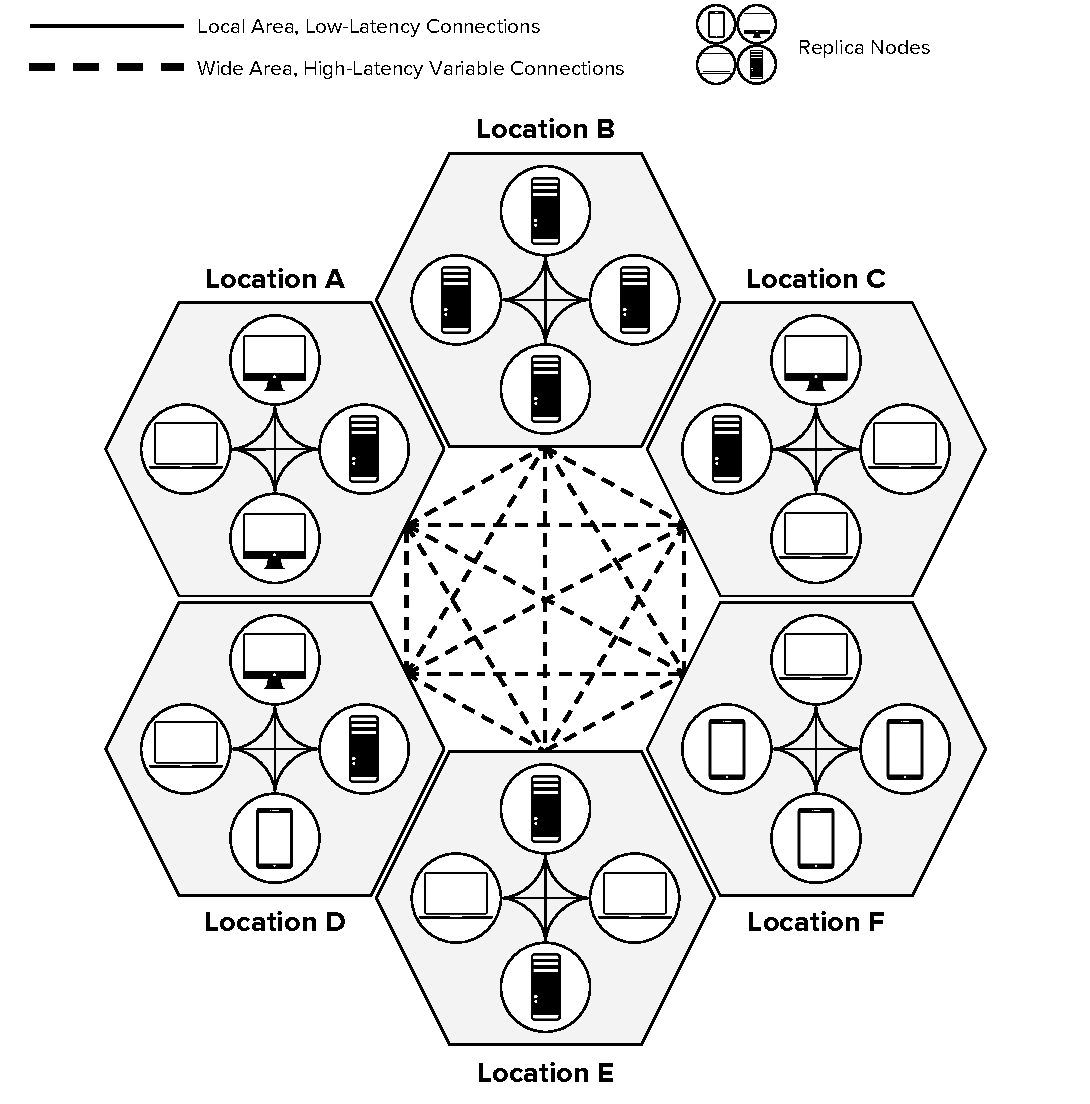
\includegraphics[width=5in]{figures/ch04_topology.pdf}
    \end{center}
    \renewcommand{\baselinestretch}{1}
    \small\normalsize

    \begin{quote}
        \caption[Simulated Federated Network Topology]{We evaluated our federated consistency model in a fully connected simulation. Each simulation specified a topology of replicas that replicas in the same region enjoyed stable, low-latency connections, while across the wide area connections were more variable. Each replica in the system is assigned a different consistency protocol to execute during runtime.}
        \label{fig:ch04_topology.pdf}
    \end{quote}
\end{figure}
\renewcommand{\baselinestretch}{2}
\small\normalsize

Input to the simulation has two parts: a network topology and a workload of access events.
The simulation instantiates each replica as a process that executes read and write accesses to objects, generates replication messages, and handles messages from other replicas.
Topologies specify each device as an independent replica by uniquely identifying it with device-specific configurations.
By far the most important configuration option is a replica's \textit{consistency} (or replication protocol), which determines the replica's behavior.
Our simulation currently defines two types of replicas:

\begin{itemize}
    \item \emph{Eventual}: Eventual replicas replicate objects with periodic anti-entropy synchronizations. During each synchronization a peer is randomly selected with two selection likelihoods, $P_{sync}$, the probability of synchronizing with a Raft replica and $P_{local}$, the ratio of local vs. wide-area peer selection.
    \item \emph{Raft}: Raft replicas implement the Raft consensus protocol, electing a leader and forwarding writes to the leader to maintain a sequential ordering of operations. Writes identified as forks of prior committed writes are dropped by whichever replica makes the identification.
\end{itemize}

The topology further specifies the \textit{location} of each device, the \textit{connections} between devices, and the \textit{distribution} of message latency on a per-connection basis.
Each connection defines the latency of messages between replicas, described as a normal distribution ($\lambda_{\mu}$, $\lambda_{\sigma}$).
There are two basic types of connections: within the local area, or across the wide area.
Connections in the local area specify a lower mean latency and less variability than connections between devices in different regions.
The tick parameter, $T$, is computed by the average worst-case latency in the simulation.
Each topology also has the capability to set runtime and device-specific configurations, though we do not take advantage of this when presenting these results.

Workloads are specified as access trace files -- time-ordered access events (reads and writes) between a specific device and a specific object name.
Each trace is constructed with a random workload generator that maps devices to accesses using a distribution of the delay between accesses, the number of objects each replica accesses, $o$, and a probability of conflict, $P_c$.
Several distributions are available, including Zipfian and uniform distributions, we are primarily interested in a high-throughput workload, therefore we used a normal distribution of access ($A_{\mu}$, $A_{\sigma}$).
Object names were assigned to replicas as follows: object names are selected and assigned to replicas, round-robin, with probability $P_c$ until each replica was assigned $o$ objects.
If $P_c = 1.0$ then every single replica would access the namespace, whereas if $P_c = 0.0$ then each replica would access a unique set of objects.
The access delay distribution was used to generate accesses to objects in
sequence, by selecting an object and reading and writing to it over time until some probability of switching objects occurred.
In effect, the final workload simulates multiple replicas reading and writing at a moderate pace for approximately one hour.

\subsection{Experiments and Metrics}
\label{ch04_experiments}

We conducted two primary experiments to test the behavior of a federated consistency system against homogeneous consensus and EC systems.
The first simulates consistency behavior in the face of increasing failure of wide-area links, in the form of region partitions.
The second explores effect of the network environment on consistency as the wide-area $\lambda_\mu$ increases.
Our simulated topology consists of twenty replicas distributed across five geographic regions.
Eventual replicas prefer to choose replicas within the same geographic region for anti-entropy, e.g. $P_{local}$ is high.
Our topology is constructed with an inner core of Raft replicas such that there is one consensus replica per region, colocated with several eventual replicas.
Our experiments were condected with synthetic access traces containing approximately 29,000 accesses (depending on the experiment), approximately two thirds of which are reads.

Our primary metrics are \textit{stale reads} and \textit{forked writes}, which produce application-visible effects.
We define forked writes as the number of writes that had more than one child (multiple writes to the same parent version), whereas reads are stale if they return anything other than the globally latest version.
We also measured \emph{write visibility}.
Recall that a write is \emph{visible} if and when it is propagated to all replicas.
Any writes that do not become fully visible (e.g. are stomped as they are propagated through the EC dissemination network) are ignored.
This metric is closely related to the \textit{percent visible} metric -- the average number of replicas a write is propagated to.
These metrics are all made possible in a simulated environment, measuring these effects in a real geo-replicated system would require a great deal of logging and data post-processing which would be error-prone due to clock synchronization errors.

\subsection{Wide Area Outages}
\label{ch04_failure_rates}

Our first simulation experiments considered the effect of outages that partitioned each simulated region so that they could not communicate with each other.
Each simulation was parameterized by a probability of failure, $P_f \in [0.0,1.0]$
The $P_f$ was used at runtime to determine if an outage was going to occur at any given timestep and the length of the outage.
A $P_f=0.5$ indicates that all wide-area links are simultaneously down (messages cannot be sent across the wide-area) 50\% of the time, whereas a $P_f=1.0$ indicates that all wide-area links are permanently down after a short initial online duration.
In the case of an outage, anti-entropy synchronizations will proceed as usual within a region, however Raft will become unavailable as every replica becomes a candidate for the duration of the outage.

\begin{figure}
    \begin{center}
        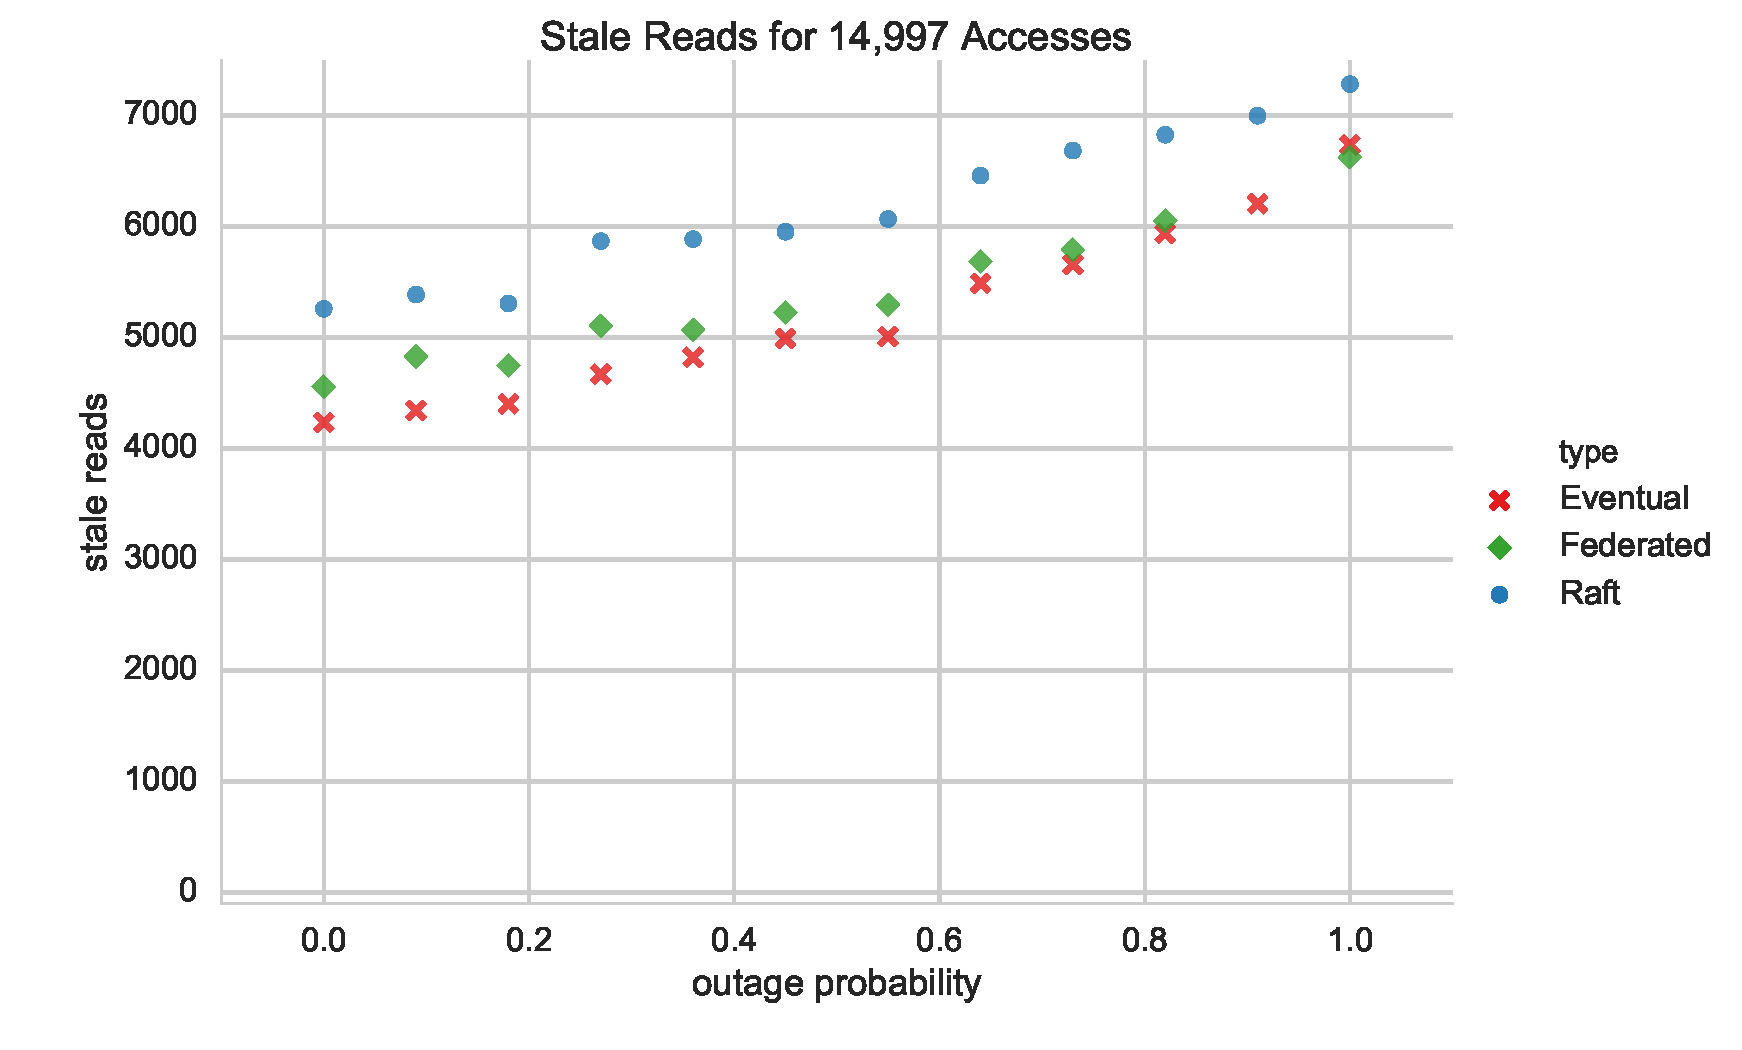
\includegraphics[width=5in]{figures/ch04_outage_stale_reads.pdf}
    \end{center}
    \renewcommand{\baselinestretch}{1}
    \small\normalsize

    \begin{quote}
        \caption[Outages Simulation Stale Reads]{Stale reads as the probability of wide-area outages increases.}
        \label{fig:ch04_outage_stale_reads}
    \end{quote}
\end{figure}
\renewcommand{\baselinestretch}{2}
\small\normalsize

\begin{figure}
    \begin{center}
        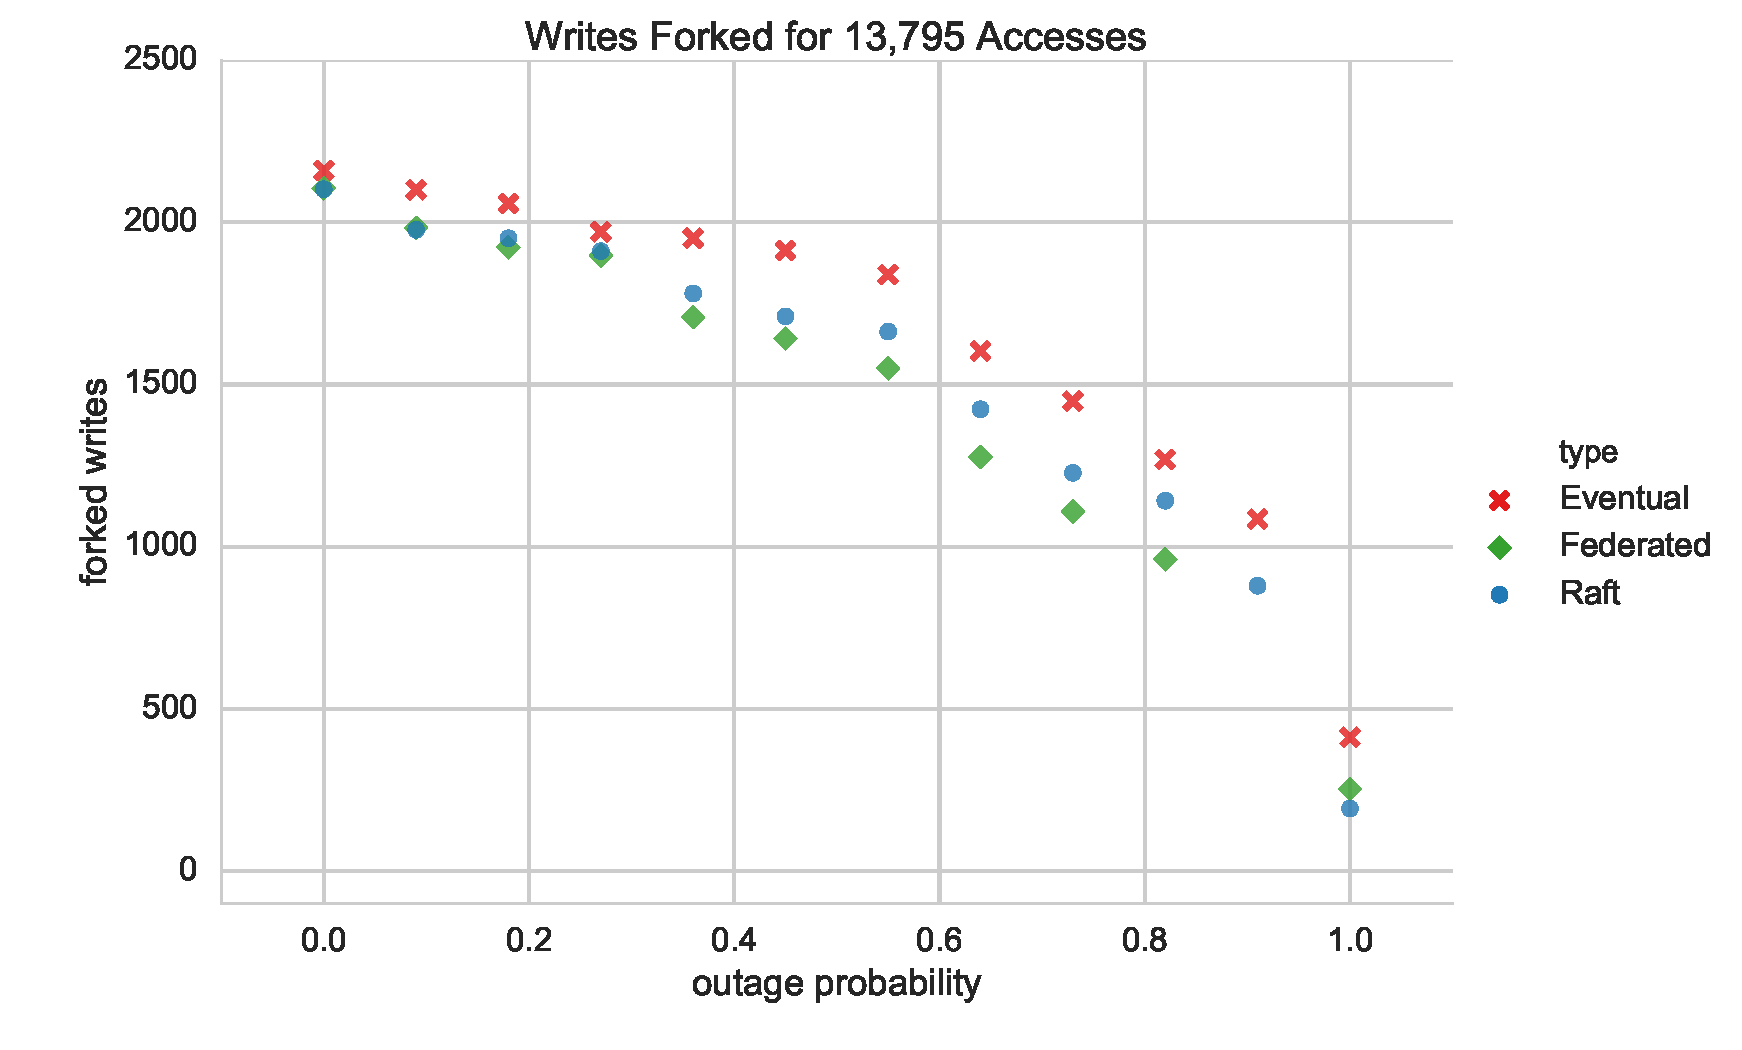
\includegraphics[width=5in]{figures/ch04_outage_forked_writes.pdf}
    \end{center}
    \renewcommand{\baselinestretch}{1}
    \small\normalsize

    \begin{quote}
        \caption[Outage Simulation Forked Writes]{Forked writes as the probability of wide-area outages increases.}
        \label{fig:ch04_outage_forked_writes}
    \end{quote}
\end{figure}
\renewcommand{\baselinestretch}{2}
\small\normalsize

We show the effect of outages on consistency by measuring stale reads in Figure~\ref{fig:ch04_outage_stale_reads} and forked writes in Figure~\ref{fig:ch04_outage_forked_writes}.
The eventual replicas deal with increasingly poor network conditions the best: randomized anti-entropy partner selection allows writes to propagate through multiple paths.
Anti-entropy and eventually consistent systems are widely used precisely because of their ability to remain highly-available during network outages.
When federated, the system is able to leverage the eventual subset of its replicas to route around failures almost as efficiently as the homogeneous Eventual system.

The multiple-paths ability also allows the federated system to propagate writes quickly, as shown in Figure~\ref{fig:ch04_outage_forked_writes}.
In fact, the federated system outperforms a homogenous eventual system, possibly because the Raft quorum is able to quickly disseminate writes during those periods when wide-area links are available.

These experiments considered complete network partitions as the failure mode, however, if the failure mode was instead random replica failures, the system would respond differently because of the way we configured the central quorum.
In a quorum size of 5, Raft can handle 2 failures before an extended outage.
Leader failure would cause temporary outages until the election timeout
occurs, but would be online with only a minimum of missed accesses.
If a Raft replica fails inside of a region, the eventually consistent replicas in that region can still make progress without the quorum.
The system also maintains the benefits of the core consensus group as synchronizations across the wide area may find a Raft replica.
Updates would still propagate across the wide area without a central broadcast mechanism at the cost of an increased number of forks as reads become increasingly stale without a local quorum component.

\subsection{Latency Variability}
\label{ch04_latency_variation}

Our second experiment investigates the effect of variable network latency on consistency protocols and how the selection of the tick parameter model affects consistency for each system.
Each simulation is parameterized by a $T$ parameter that is a function of the wide area $\lambda_{\mu}$ and $\lambda_{\sigma}$.
We used the same workload trace across all simulations, fixing the access mean, $A_\mu=3000$, e.g. approximately one access per replica every 3 seconds.
In effect, this meant that for approximately half the simulations (with higher latencies), it was impossible for a write to become visible on another replica before a fork.
The probability of conflict for the workload was set to $P_c=0.5$, however, there was still enough conflict due to connection latencies to force each protocol to handle many forks.

\begin{figure}
    \begin{center}
        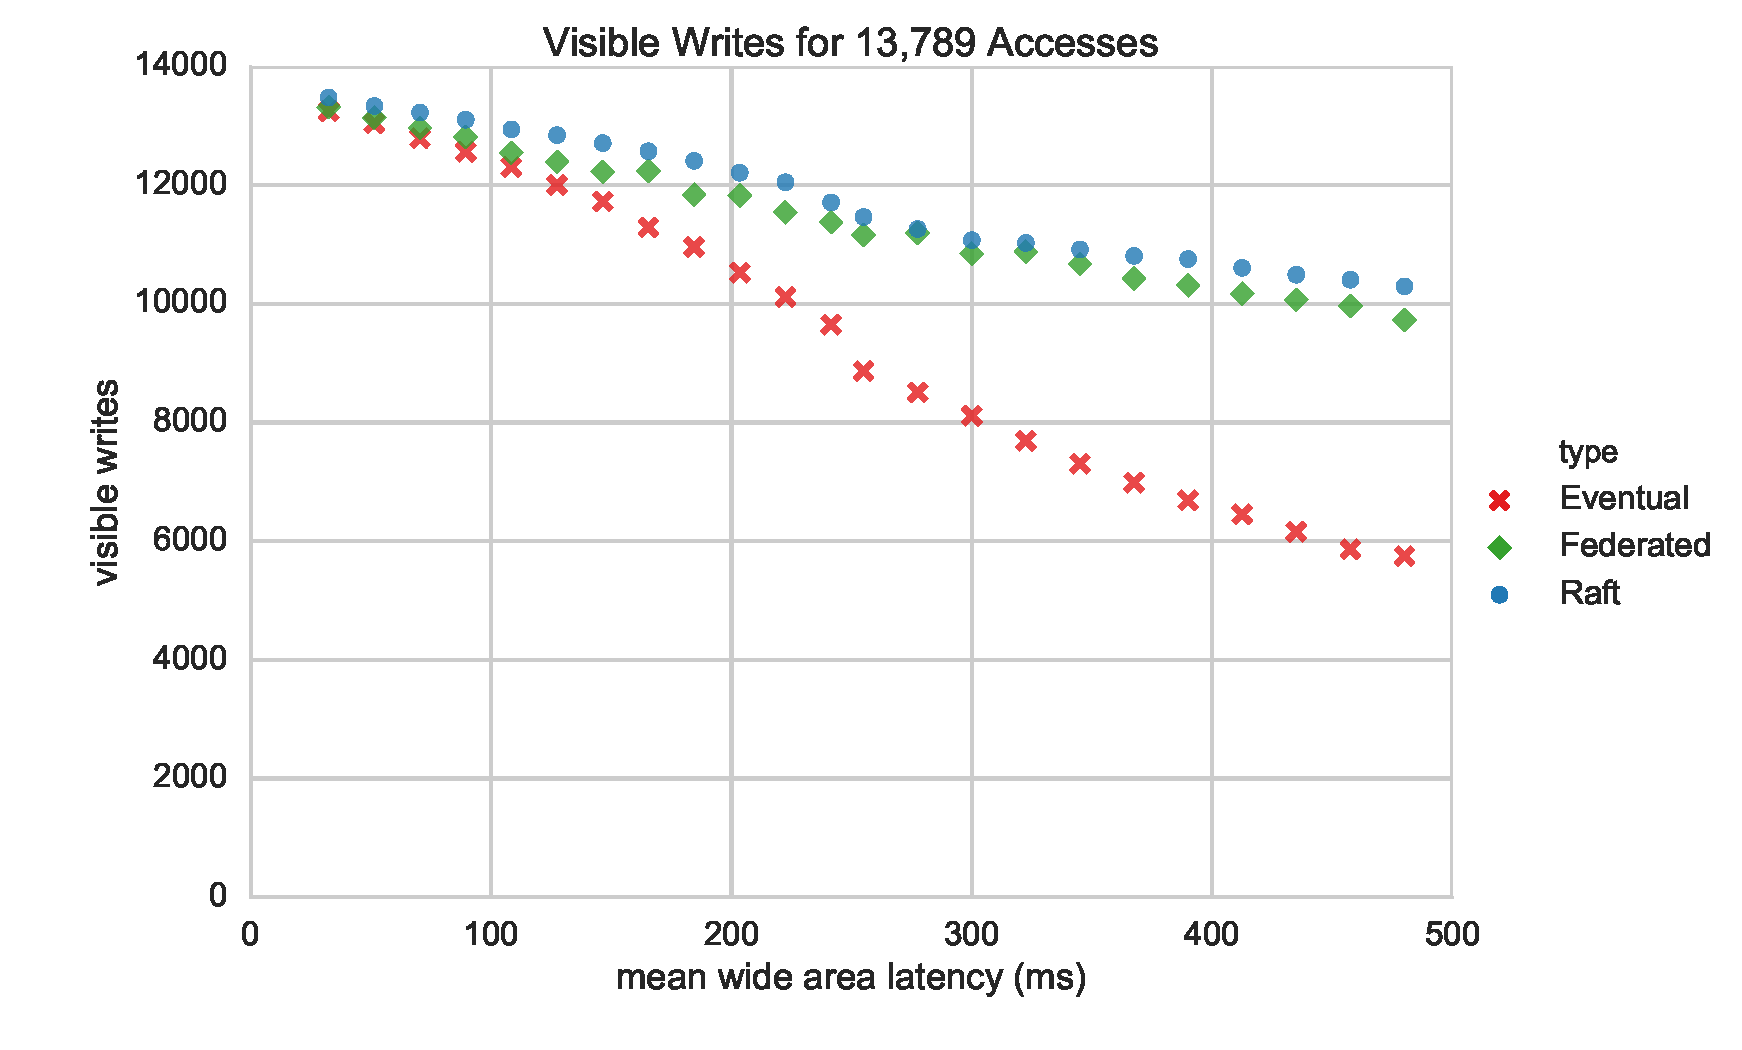
\includegraphics[width=5in]{figures/ch04_latency_visible_writes.pdf}
    \end{center}
    \renewcommand{\baselinestretch}{1}
    \small\normalsize

    \begin{quote}
        \caption[Latency Simulation Visible Writes]{The percentage of fully visible writes as the mean wide area latency increases.}
        \label{fig:ch04_latency_visible_writes}
    \end{quote}
\end{figure}
\renewcommand{\baselinestretch}{2}
\small\normalsize

\begin{figure}
    \begin{center}
        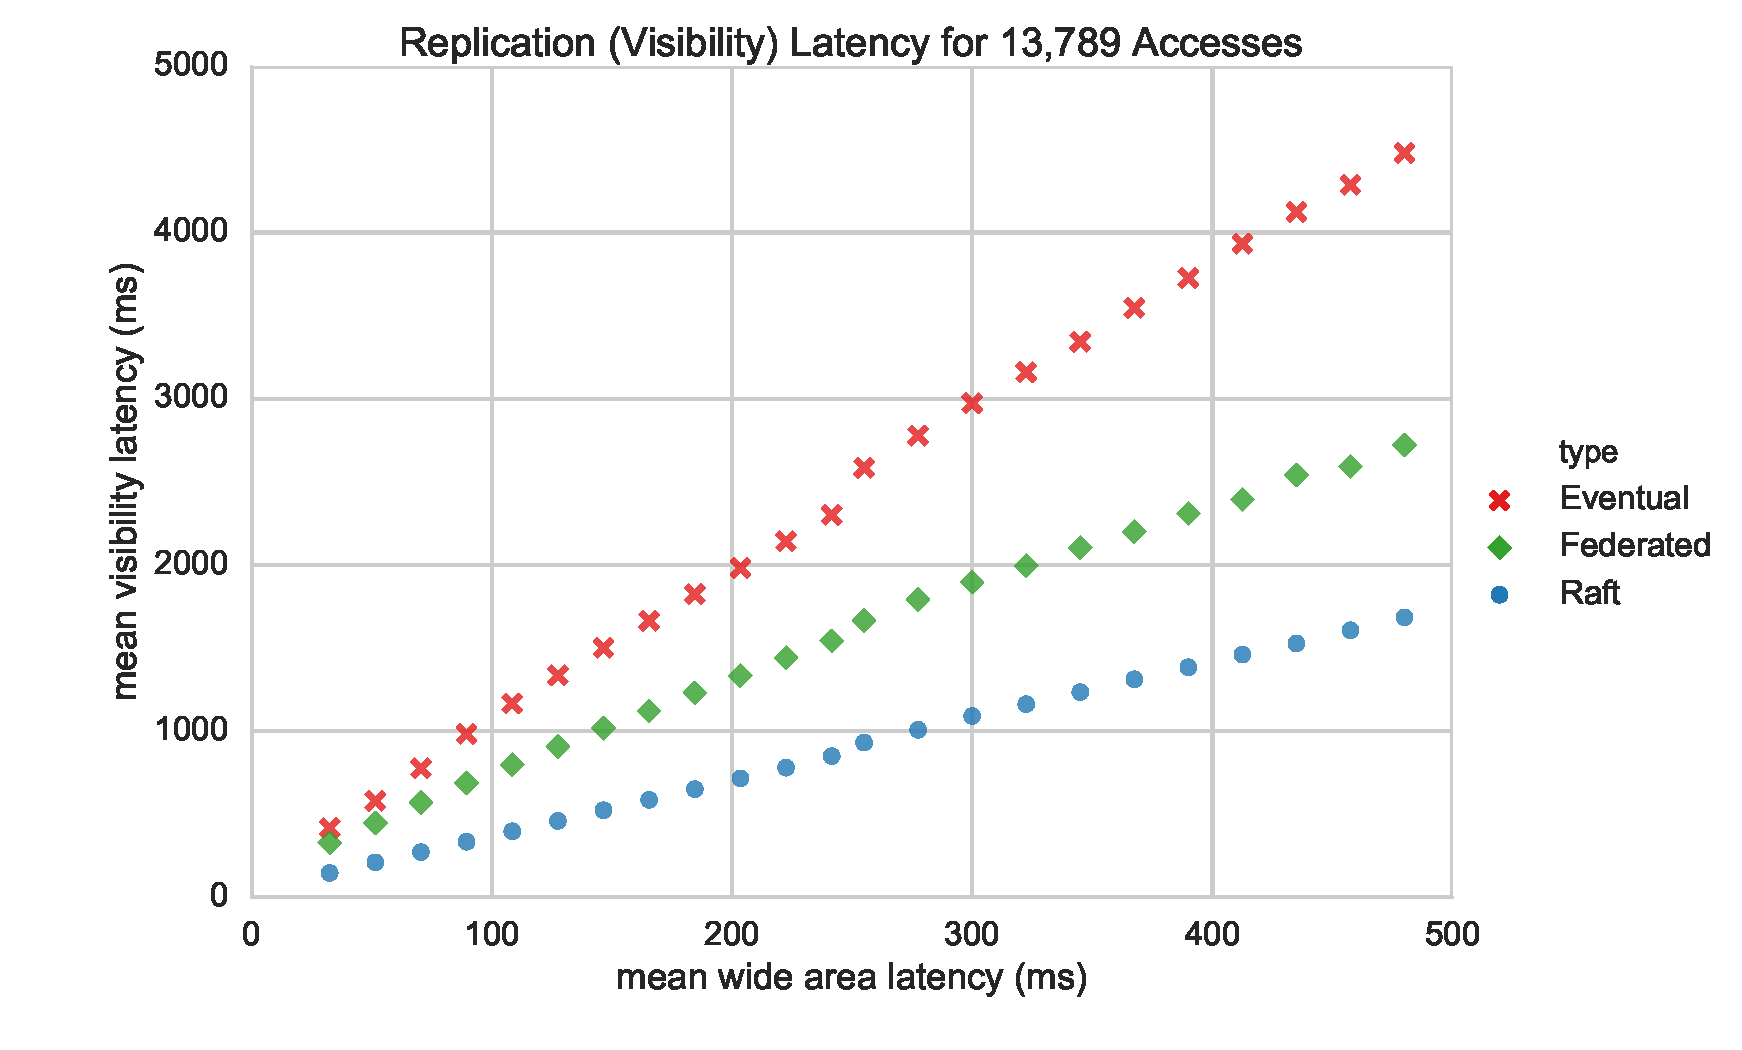
\includegraphics[width=5in]{figures/ch04_latency_visibility_latency.pdf}
    \end{center}
    \renewcommand{\baselinestretch}{1}
    \small\normalsize

    \begin{quote}
        \caption[Latency Simulation Visibility Latency]{The average amount of time an update becomes fully visible (if the update becomes fully visible).}
        \label{fig:ch04_latency_visibility_latency}
    \end{quote}
\end{figure}
\renewcommand{\baselinestretch}{2}
\small\normalsize

Figures~\ref{fig:ch04_latency_visible_writes} and \ref{fig:ch04_latency_visibility_latency} show that write propagation is much faster and more effective in Raft than in eventual, especially as network conditions deteriorate.
Raft ensures that writes become fully replicated at the cost of increased write latencies, moreover they require broadcast over the wide area.
This is not an ideal scenario in failure prone networks, but broadcast from a single leader ensures propagation is fast.
Federated essentially splits the difference between Raft and eventual in terms of mean replication latency.
However, Figure~\ref{fig:ch04_latency_visible_writes} shows that federated fully replicates many more writes than eventual, closely tracking the number of writes fully replicated by Raft.

The strong inner core of Raft replicas is the key to the federated protocol tracking Raft's performance.
EC replicas are biased in favor of performing anti-entropy with local replicas, allowing most anti-entropy sessions to perform quickly and without delay.
By contrast, the Raft replicas in the federated topology are intentionally spread across geographic regions.
A new write originating at an eventual replica is quickly spread to the local
Raft replica, and is then broadcast to the rest of the regions via consensus decisions.
Disseminating writes quickly minimizes the possibility of another, later
eventual write starting up concurrently.
Additionally, the forte number prevents new forked writes from stomping on a
conflicting write disseminated via Raft replicas.

\begin{figure}
    \begin{center}
        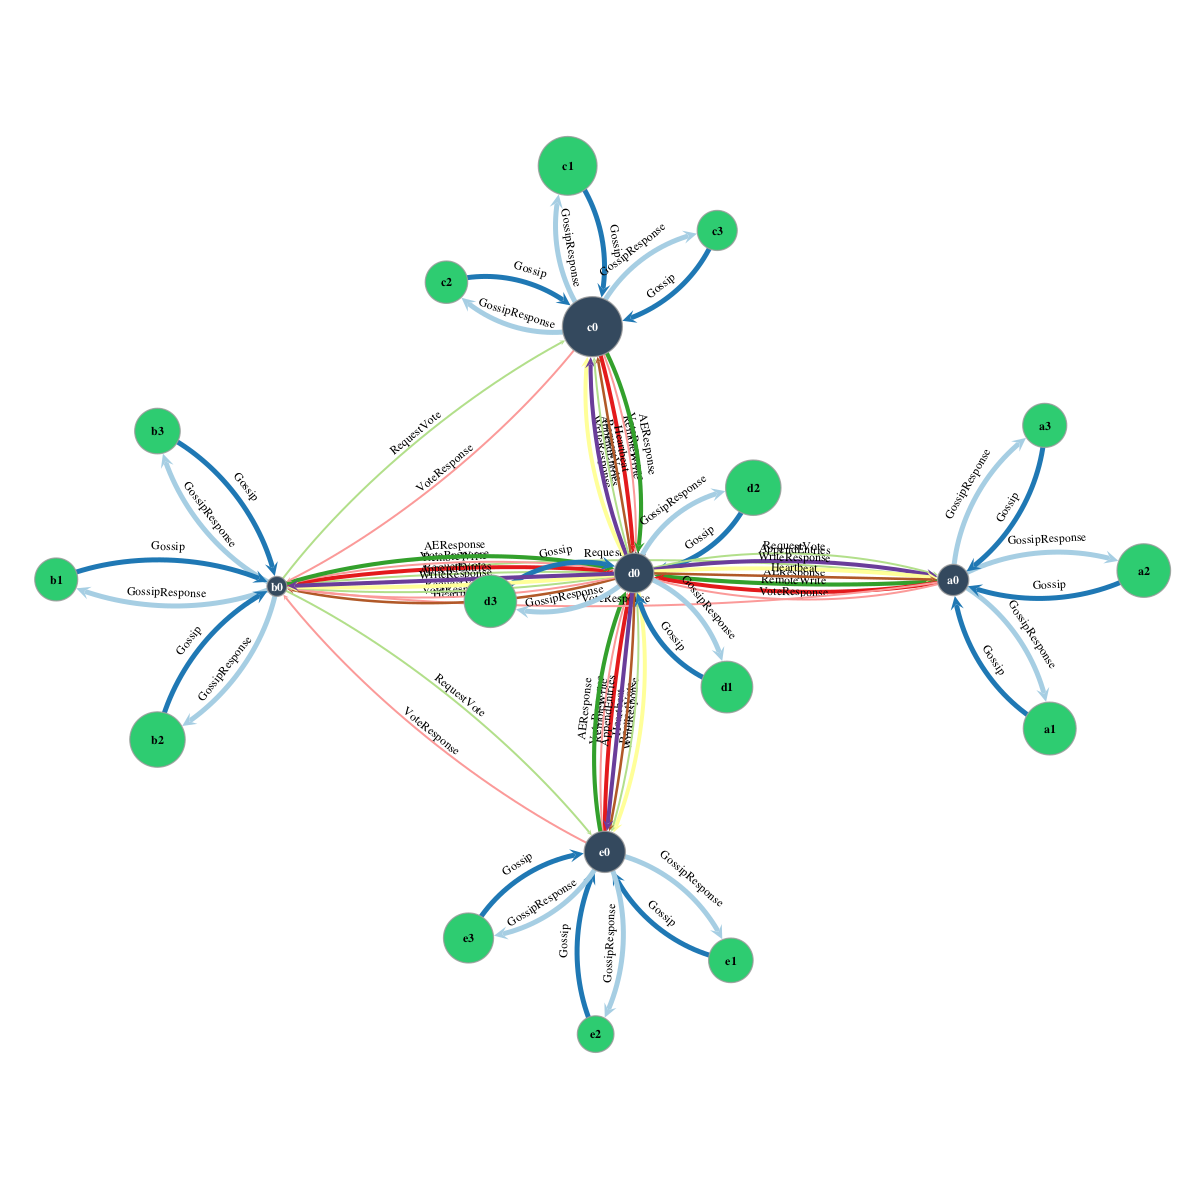
\includegraphics[width=5in]{figures/ch04_federated_sync.png}
    \end{center}
    \renewcommand{\baselinestretch}{1}
    \small\normalsize

    \begin{quote}
        \caption[Federated Syncronization Topology]{This graph shows the synchronization of a federated topology for a simulation run that optimizes Raft connections in the wide area and eventual connections in the local area. Vertex size indicates the number of accesses at each replica and color represents the replica type (blue for Raft, green for eventual). Edges are colored by RPC type and sized by the number of messages sent.}
        \label{fig:ch04_federated_sync}
    \end{quote}
\end{figure}
\renewcommand{\baselinestretch}{2}
\small\normalsize

The effect of Raft disseminating updates across the wide area can be seen in access network extracted from our simulation shown in Figure~\ref{fig:ch04_federated_sync}.
In this network, vertices represent replicas and are colored by the consistency protocol it implements (blue for Raft, green for eventual).
The size of the vertex represents the number of accesses that occur at each location.
The edges are colored by RPC type and are sized by the number of message of that type sent between replicas.
This network shows an extreme optimization of a federated network, using Raft as a broadcast network across the wide area and local synchronization to anti-entropy nodes.
Although this type of network did not perform as well in the outage simulations, it performed very well for our variable latency simulations.
These observations served as the basis for our planetary architecture as described in \S~\ref{ch02_planetary_scale_architecture}.

Figures~\ref{fig:ch04_latency_stale_reads} and \ref{fig:ch04_latency_forked_writes} show the average number of stale reads and forked writes across different mean latencies.
All three protocols perform similarly at smaller latencies, but eventual and federated deal with high latencies much more effectively than Raft, at least
for this size of system.

\begin{figure}
    \begin{center}
        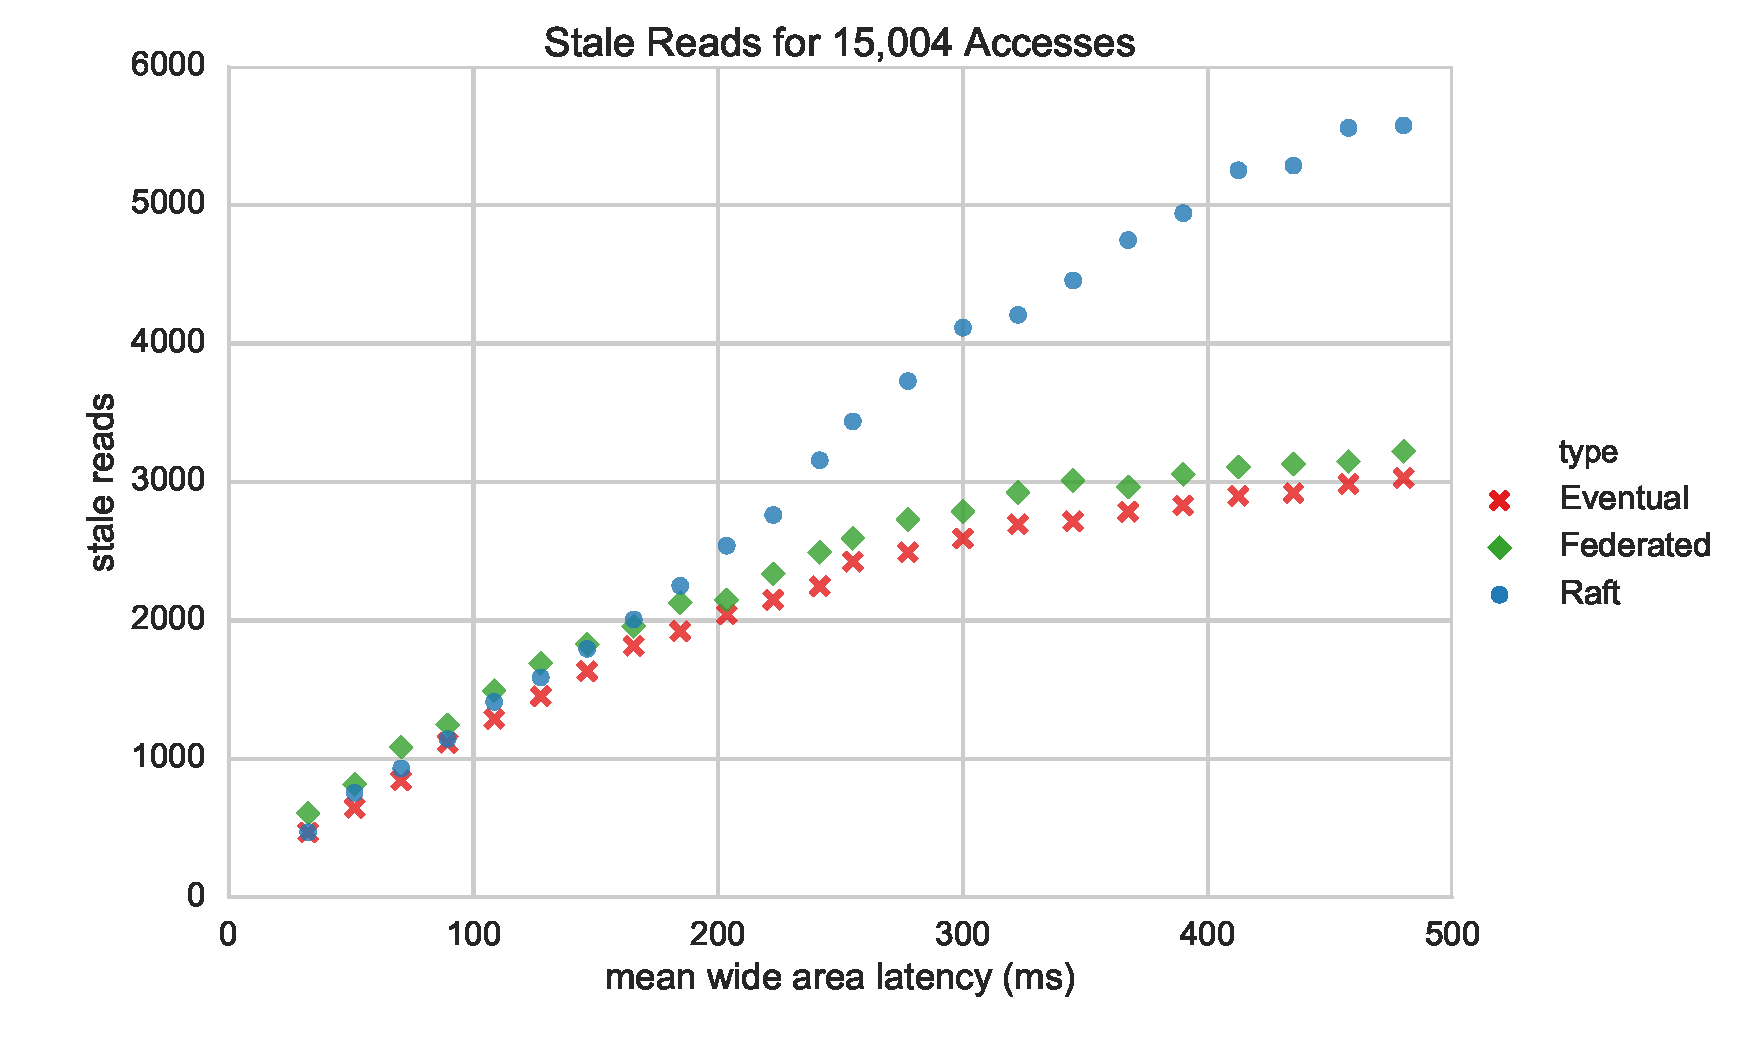
\includegraphics[width=5in]{figures/ch04_latency_stale_reads.pdf}
    \end{center}
    \renewcommand{\baselinestretch}{1}
    \small\normalsize

    \begin{quote}
        \caption[Latency Simulation Stale Reads]{The total number of reads that are stale when they are executed.}
        \label{fig:ch04_latency_stale_reads}
    \end{quote}
\end{figure}
\renewcommand{\baselinestretch}{2}
\small\normalsize

\begin{figure}
    \begin{center}
        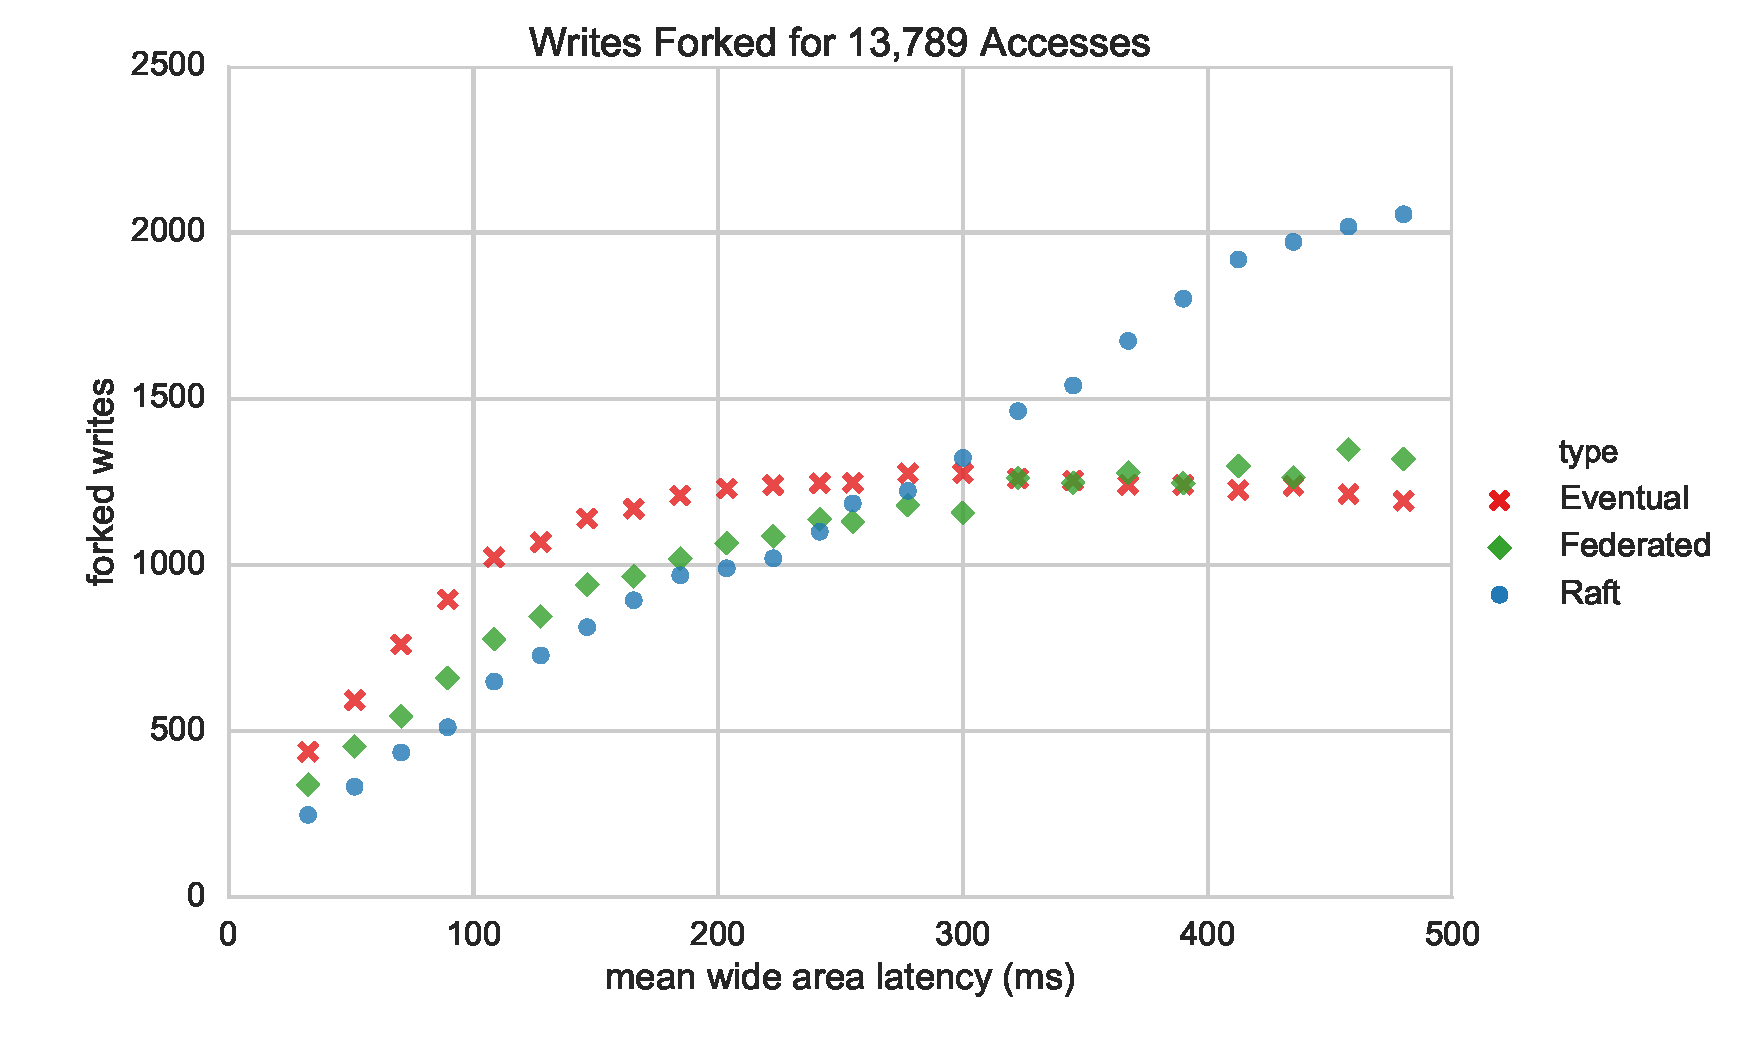
\includegraphics[width=5in]{figures/ch04_latency_forked_writes.pdf}
    \end{center}
    \renewcommand{\baselinestretch}{1}
    \small\normalsize

    \begin{quote}
        \caption[Latency Simulation Forked Writes]{The total number of writes that are forked, potential application-level conflicts.}
        \label{fig:ch04_latency_forked_writes}
    \end{quote}
\end{figure}
\renewcommand{\baselinestretch}{2}
\small\normalsize

Higher latencies affect Raft in at least two ways.
First, higher latency variability causes more out of order messages.
Second, system timeouts are parameterized by $T$ which, in turn, is based on mean latencies.
The result is that Raft's append entries delay is longer for simulations with higher mean latencies, resulting in more conflicts.
The same is true for anti-entropy delays, but the speed of Raft decisions is determined by the slowest quorum member, which can be quite slow when message variability is large.
By contrast, a slow anti-entropy participant only affects direct anti-entropy partners, not the replication of the update across the whole system.

Though not shown here, we also investigated the effect of changing the number of replicas in the system (a system implementation shows that consensus does not scale well in Figure~\ref{fig:ch03_scaling_consensus}).
As system size increases, more time is required to fully replicate writes, increasing the likelihood of both stale reads and forks.
Equation~\ref{eq:anti_entropy_visibility_latency} shows that bilateral anti-entropy propagates writes to $N$ nodes exponentially.
Given the relationship of the \texttt{anti-entropy delay} and \texttt{heartbeat interval} expressed by $T$, Raft broadcasts overtake anti-entropy between 9 (2 anti-entropy sessions) and 27 replicas (3 anti-entropy sessions).

Finally, Figure~\ref{fig:ch04_latency_write_latency} shows the mean synchronous cost of write operations to ongoing computations.
All Raft writes must be forwarded to the leader to be serialized and are completed after a round trip communication.
Eventual writes are local and are completed immediately, even before being replicated, and therefore have zero write cost.
Most federated replicas are eventual and therefore federated's average write cost tracks eventual's relatively closely.

\begin{figure}
    \begin{center}
        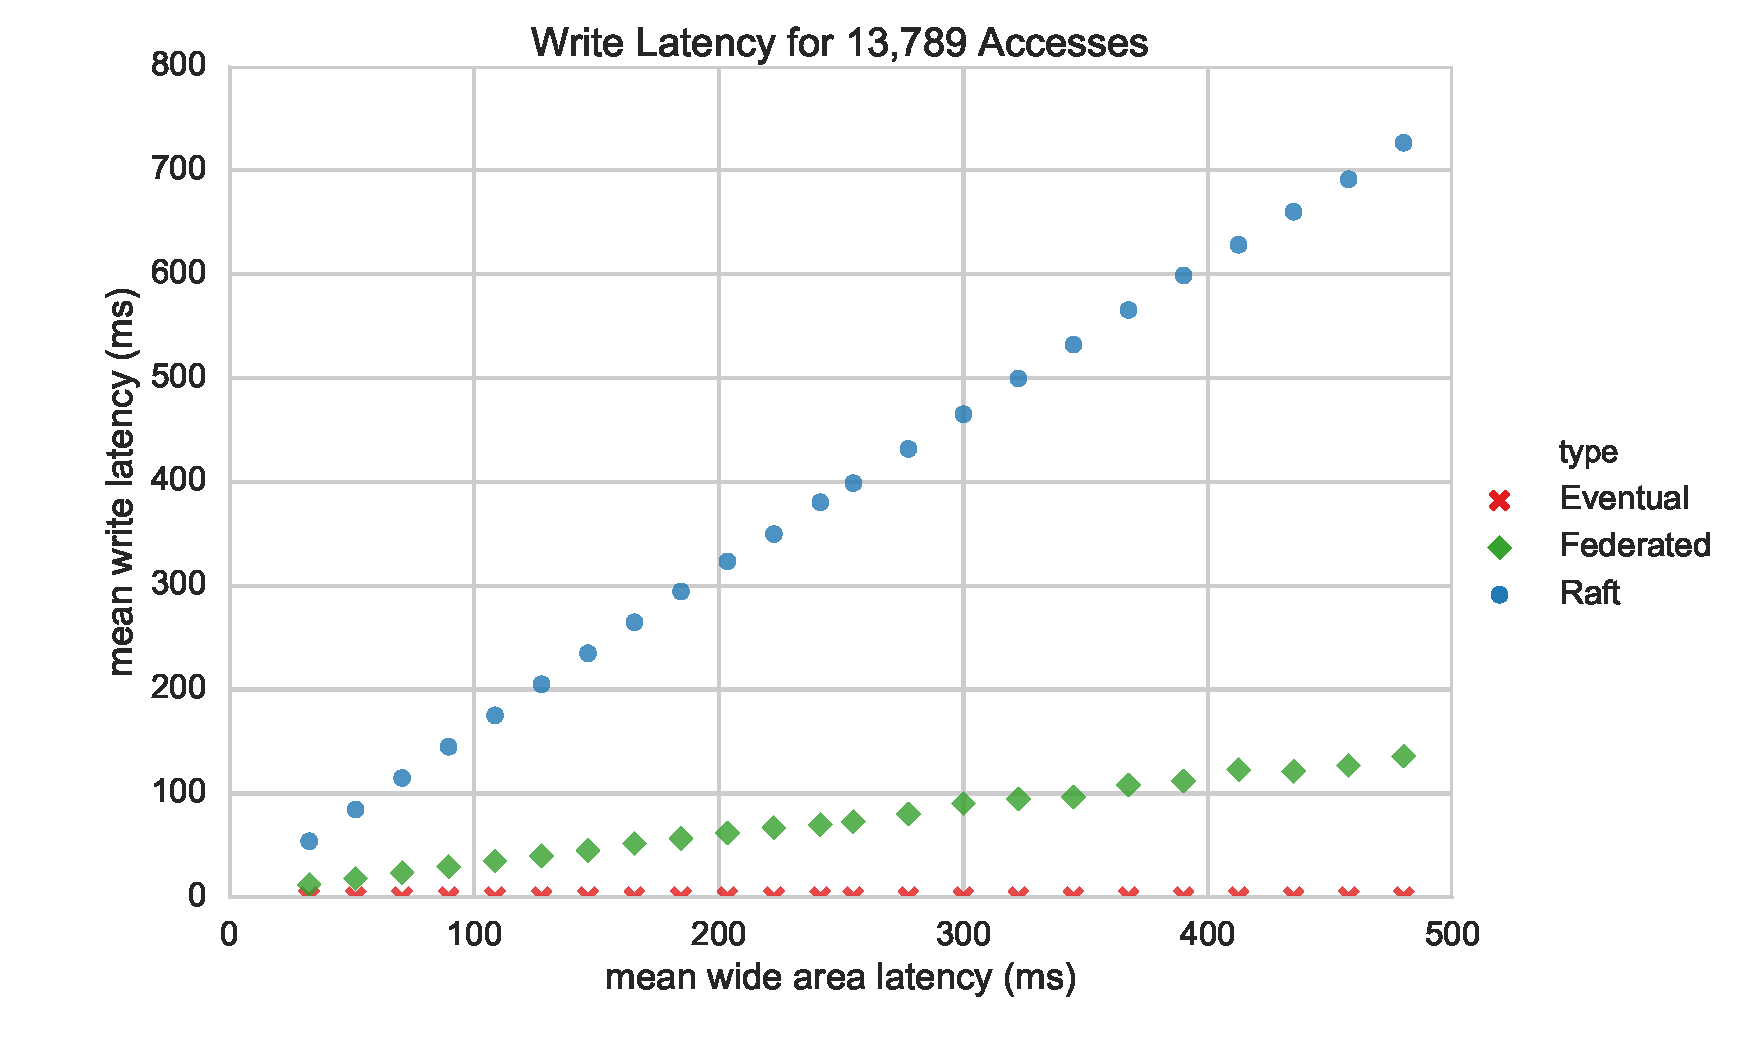
\includegraphics[width=5in]{figures/ch04_latency_write_latency.pdf}
    \end{center}
    \renewcommand{\baselinestretch}{1}
    \small\normalsize

    \begin{quote}
        \caption[Latency Simulation Write Latency]{Average cost of writes to local replicas. Eventual consistency writes are completed immediately without coordination, therefore have zero cost. The cost of Raft depends on the latency of the majority vote. Federated with more eventual replicas will more than halve the average write cost in the system.}
        \label{fig:ch04_latency_write_latency}
    \end{quote}
\end{figure}
\renewcommand{\baselinestretch}{2}
\small\normalsize

\section{Conclusion}
\label{ch04_conclusion}

In this chapter we have presented a model for federated consistency to hybridize consistency protocols in a single system.
Federated consistency allows individual replicas to expose local consistency policies to users, while still allowing for global guarantees.
We explored the federation of eventual consistency implemented with anti-entropy synchronization and sequential consistency implemented with Raft consensus.

Federation requires both communication and consistency integration at the consistency boundary, that is when replicas of different policies interact.
We solved communication integration by identifying how each consensus protocol should respond to RPCs of the other, and by introducing parameters that modified how peers were selected to communicate with each other.
Consistency integration involved ensuring that decisions made by either protocol were respected by the other.
By default this is not the case, since each protocol selected writes in opposite ways.
We therefore had to have a way for each protocol to determine the most relevant write to propagate, which we solved by extending conflict-free version numbers with a forte number that could only be incremented by the Raft leader.
Though we only investigated eventual and sequential consistency, we propose that other consistency models, e.g. causal consistency, could be similarly federated.

We evaluated federated consistency in the context of a geographically dispersed wide-area object store using a simulation to track metrics not generally available in a real implementation.
Our results show that a key to the global guarantees is using a core consensus group to serialize and broadcast system writes.
By designing a federated system where only interactions between replicas of varying consistency types are defined, systems can scale beyond the handful of devices usually described to dozens or hundreds of replicas in variable-latency, partition-prone geographic networks.
Replicas can monitor their local environment and adapt as necessary to meet timeliness and correctness constraints required by the local user.

We were only able to investigate a limited number of system configurations.
However, the space of possible system configurations is vast.
We do not claim that the configurations described in this chapter are in any way optimal.
Rather, we claim that the extremely promising results described in
Section~\ref{sec:results} show that the general approach is promising.
Our simulation environment is extremely flexible, and we intend to continue
evaluating possible system configurations in parallel with our system development.

Federated consistency has the potential to scale system sizes to extremely large networks of millions of nodes.
For this to happen our ideal configuration using a central Raft quorum must also scale, which is possible when using hierarchical consensus.
Planetary scale systems comprised of a fog of highly available, eventually consistent replicas federated with a central core of strong consistency hierarchical consensus will allow high throughput, rapid replication, high availability, and resistance to outages and variable network conditions.
